\documentclass[twoside]{book}

% Packages required by doxygen
\usepackage{fixltx2e}
\usepackage{calc}
\usepackage{doxygen}
\usepackage[export]{adjustbox} % also loads graphicx
\usepackage{graphicx}
\usepackage[utf8]{inputenc}
\usepackage{makeidx}
\usepackage{multicol}
\usepackage{multirow}
\PassOptionsToPackage{warn}{textcomp}
\usepackage{textcomp}
\usepackage[nointegrals]{wasysym}
\usepackage[table]{xcolor}

% Font selection
\usepackage[T1]{fontenc}
\usepackage[scaled=.90]{helvet}
\usepackage{courier}
\usepackage{amssymb}
\usepackage{sectsty}
\renewcommand{\familydefault}{\sfdefault}
\allsectionsfont{%
  \fontseries{bc}\selectfont%
  \color{darkgray}%
}
\renewcommand{\DoxyLabelFont}{%
  \fontseries{bc}\selectfont%
  \color{darkgray}%
}
\newcommand{\+}{\discretionary{\mbox{\scriptsize$\hookleftarrow$}}{}{}}

% Page & text layout
\usepackage{geometry}
\geometry{%
  a4paper,%
  top=2.5cm,%
  bottom=2.5cm,%
  left=2.5cm,%
  right=2.5cm%
}
\tolerance=750
\hfuzz=15pt
\hbadness=750
\setlength{\emergencystretch}{15pt}
\setlength{\parindent}{0cm}
\setlength{\parskip}{3ex plus 2ex minus 2ex}
\makeatletter
\renewcommand{\paragraph}{%
  \@startsection{paragraph}{4}{0ex}{-1.0ex}{1.0ex}{%
    \normalfont\normalsize\bfseries\SS@parafont%
  }%
}
\renewcommand{\subparagraph}{%
  \@startsection{subparagraph}{5}{0ex}{-1.0ex}{1.0ex}{%
    \normalfont\normalsize\bfseries\SS@subparafont%
  }%
}
\makeatother

% Headers & footers
\usepackage{fancyhdr}
\pagestyle{fancyplain}
\fancyhead[LE]{\fancyplain{}{\bfseries\thepage}}
\fancyhead[CE]{\fancyplain{}{}}
\fancyhead[RE]{\fancyplain{}{\bfseries\leftmark}}
\fancyhead[LO]{\fancyplain{}{\bfseries\rightmark}}
\fancyhead[CO]{\fancyplain{}{}}
\fancyhead[RO]{\fancyplain{}{\bfseries\thepage}}
\fancyfoot[LE]{\fancyplain{}{}}
\fancyfoot[CE]{\fancyplain{}{}}
\fancyfoot[RE]{\fancyplain{}{\bfseries\scriptsize Generated by Doxygen }}
\fancyfoot[LO]{\fancyplain{}{\bfseries\scriptsize Generated by Doxygen }}
\fancyfoot[CO]{\fancyplain{}{}}
\fancyfoot[RO]{\fancyplain{}{}}
\renewcommand{\footrulewidth}{0.4pt}
\renewcommand{\chaptermark}[1]{%
  \markboth{#1}{}%
}
\renewcommand{\sectionmark}[1]{%
  \markright{\thesection\ #1}%
}

% Indices & bibliography
\usepackage{natbib}
\usepackage[titles]{tocloft}
\setcounter{tocdepth}{3}
\setcounter{secnumdepth}{5}
\makeindex

% Hyperlinks (required, but should be loaded last)
\usepackage{ifpdf}
\ifpdf
  \usepackage[pdftex,pagebackref=true]{hyperref}
\else
  \usepackage[ps2pdf,pagebackref=true]{hyperref}
\fi
\hypersetup{%
  colorlinks=true,%
  linkcolor=blue,%
  citecolor=blue,%
  unicode%
}

% Custom commands
\newcommand{\clearemptydoublepage}{%
  \newpage{\pagestyle{empty}\cleardoublepage}%
}

\usepackage{caption}
\captionsetup{labelsep=space,justification=centering,font={bf},singlelinecheck=off,skip=4pt,position=top}

%===== C O N T E N T S =====

\begin{document}

% Titlepage & ToC
\hypersetup{pageanchor=false,
             bookmarksnumbered=true,
             pdfencoding=unicode
            }
\pagenumbering{alph}
\begin{titlepage}
\vspace*{7cm}
\begin{center}%
{\Large Tokenika eosc }\\
\vspace*{1cm}
{\large Generated by Doxygen 1.8.13}\\
\end{center}
\end{titlepage}
\clearemptydoublepage
\pagenumbering{roman}
\tableofcontents
\clearemptydoublepage
\pagenumbering{arabic}
\hypersetup{pageanchor=true}

%--- Begin generated contents ---
\chapter{Tokenika alternative for the E\+OS $\ast$eosc$\ast$ program}
\label{md__r_e_a_d_m_e}
\Hypertarget{md__r_e_a_d_m_e}
\subsection*{Rationale}

For our work with eos small contracts, we have found that the original E\+OS {\ttfamily eosc} interface program is too much restrictive. First, it is hard to be used programmatically in a C++ code. Next, it is quite heavy as it is tightly connected to the whole of the E\+OS code. Also, it is not ready to be used in the Windows environment, while we plan to open Windows based contract development possibility.

It could be enough for us to develope a minimal C++ library, implementing the commands of the E\+OS {\ttfamily eosc}. However, it was a short step to to provide this library with an command line interface.

Finally, to make our work competitive to the original, and for fun, we have added a richer command option list. We dare to hope that this little work of ours could be included to the E\+OS project.

We already know how to use this richness\+: it is much ease to make a tool as tokenika \href{#}{\tt {\ttfamily eosc\+Bash}} that wraps the E\+OS {\ttfamily eosc} for bookkeeping.

\subsection*{Richer A\+PI}

\#\#\# E\+OS 
\begin{DoxyCode}
./eosc get block -h
\end{DoxyCode}
 
\begin{DoxyCode}
ERROR: RequiredError: block
Retrieve a full block from the blockchain
Usage: ./eosc get block block

Positionals:
  block TEXT                  The number or ID of the block to retrieve
\end{DoxyCode}
 
\begin{DoxyCode}
./eosc get block 25
\end{DoxyCode}
 
\begin{DoxyCode}
\{
  "previous": "00000018b5e0ffcd3dfede45bc261e3a04de9f1f40386a69821780e063a41448",
  "timestamp": "2017-11-29T09:50:03",
  "transaction\_merkle\_root": "0000000000000000000000000000000000000000000000000000000000000000",
  "producer": "initf",
  "producer\_changes": [],
  "producer\_signature":
       "2005db1a193cc3597fdc3bd38a4375df2a9f9593390f9431f7a9b53701cd46a1b5418b9cd68edbdf2127d6ececc4d66b7a190e72a97ce9adfcc750ef0a770f5619",
  "cycles": [],
  "id": "000000190857c9fb43d62525bd29dc321003789c075de593ce7224bde7fc2284",
  "block\_num": 25,
  "refBlockPrefix": 623236675
\}
\end{DoxyCode}


\subsubsection*{Tokenika}


\begin{DoxyCode}
./eosc get block -h
\end{DoxyCode}
 
\begin{DoxyCode}
Retrieve a full block from the blockchain
Usage: ./eosc get block [block\_num] [Options]
Usage: ./eosc get block [-j \{"block\_num\_or\_id":*\}] [OPTIONS]

Options:

  -n [ --block\_num ] arg  Block number
  -i [ --block\_id ] arg   Block id

  -h [ --help ]           Help screen
  -j [ --json ] arg       Json argument
  -v [ --received ]       Print received json
  -r [ --raw ]            Not pretty print
  -e [ --example ]        Usage example
\end{DoxyCode}
 
\begin{DoxyCode}
./eosc get block 25
##         block number: 25
##            timestamp: 2017-11-29T09:50:03
##     ref block prefix: 623236675
\end{DoxyCode}
 
\begin{DoxyCode}
./eosc get block 25 -v
\end{DoxyCode}
 
\begin{DoxyCode}
\{
    "previous": "00000018b5e0ffcd3dfede45bc261e3a04de9f1f40386a69821780e063a41448",
    "timestamp": "2017-11-29T09:50:03",
    "transaction\_merkle\_root": "0000000000000000000000000000000000000000000000000000000000000000",
    "producer": "initf",
    "producer\_changes": "",
    "producer\_signature":
       "2005db1a193cc3597fdc3bd38a4375df2a9f9593390f9431f7a9b53701cd46a1b5418b9cd68edbdf2127d6ececc4d66b7a190e72a97ce9adfcc750ef0a770f5619",
    "cycles": "",
    "id": "000000190857c9fb43d62525bd29dc321003789c075de593ce7224bde7fc2284",
    "block\_num": "25",
    "refBlockPrefix": "623236675"
\}
\end{DoxyCode}
 
\begin{DoxyCode}
./eosc get block 25 -v -r
\end{DoxyCode}
 
\begin{DoxyCode}

      \{"previous":"00000018b5e0ffcd3dfede45bc261e3a04de9f1f40386a69821780e063a41448","timestamp":"2017-11-29T09:50
      :03","transaction\_merkle\_root":"0000000000000000000000000000000000000000000000000000000000000000","producer"
      :"initf","producer\_changes":"","producer\_signature":"2005db1a193cc3597fdc3bd38a4375df2a9f9593390f9431f7a9b53
      701cd46a1b5418b9cd68edbdf2127d6ececc4d66b7a190e72a97ce9adfcc750ef0a770f5619","cycles":"","id":"000000190857c9fb43d62525bd29dc321003789c075de593ce7224bde7fc2284","block\_num":"25","refBlockPrefix":"623236675"\}
\end{DoxyCode}
 
\begin{DoxyCode}
./eosc get block -j '\{"block\_num\_or\_id":"56"\}'
##         block number: 56
##            timestamp: 2017-11-29T10:02:18
##     ref block prefix: 273573026
\end{DoxyCode}
 
\begin{DoxyCode}
./eosc get block --example
\end{DoxyCode}
 
\begin{DoxyCode}
Invoke 'GetInfo' command:
GetInfo GetInfo;

\{
    "head\_block\_num": "9939",
    "last\_irreversible\_block\_num": "9924",
    "head\_block\_id": "000026d378f90b5d25dcf962fc44d637872218e5f826420a342f05a534d50bfc",
    "head\_block\_time": "2017-12-01T18:57:42",
    "head\_block\_producer": "initr",
    "recent\_slots": "0000000000000000000000000000000000000000000000000011111111111111",
    "participation\_rate": "0.21875000000000000"
\}


Use reference to the last block:
GetBlock GetBlock(
  GetInfo.get<int>("last\_irreversible\_block\_num"));

\{
    "previous": "000026c35fb5d442be6d4e81a1347cce2c0184c4c2047d9e6dfc78b3bb325ac2",
    "timestamp": "2017-12-01T17:01:09",
    "transaction\_merkle\_root": "0000000000000000000000000000000000000000000000000000000000000000",
    "producer": "initn",
    "producer\_changes": "",
    "producer\_signature":
       "1f6984d14ee40ed9806ae14aa96531d874fc3417bf3f1b66c4b1d9c9402f3f90ef07c4523eb9a639ad632c181580aeb051385d718dc59ecc54d0f0e5de012b540f",
    "cycles": "",
    "id": "000026c44a2e8075a5b92813869bfb67b72b79ccb3f2e40ad815603c04d2fafd",
    "block\_num": "9924",
    "refBlockPrefix": "321436069"
\}
\end{DoxyCode}
 \subsection*{Library}

For us, a real value is the library that runs the tokenika\+::eosc, as we see the original eos library as not practical for our work. We need a light-\/weight thing, a cross-\/platform (good for windows) one.

Let you see a code snippet\+: 
\begin{DoxyCode}
#include <stdio.h>
#include <stdlib.h>
#include <iostream>
#include <string>

#include "EoscCommands/eosc\_get\_commands.hpp"

int main(int argc, char *argv[])
\{
  tokenika::eosc::GetInfo GetInfo; /* Call 'eosd' for 'get info'. */
  tokenika::eosc::GetBlock GetBlock( /* Call 'eosd' for 'get block', the last one. */
    GetInfo.get<int>("last\_irreversible\_block\_num"));

  std::cout << GetBlock.to\_string\_rcv() << std::endl;/* Print the response. */

  return 0;
\}
\end{DoxyCode}
 Here is the print-\/out\+: 
\begin{DoxyCode}
    "previous": "000028716589219b442afe9d140bc28eff4335aecd37d519b0105fca4c8e4a3f",
    "timestamp": "2017-12-01T19:18:27",
    "transaction\_merkle\_root": "0000000000000000000000000000000000000000000000000000000000000000",
    "producer": "inith",
    "producer\_changes": "",
    "producer\_signature":
       "1f510dec0bcd85847b7bead61f6deee7a5fb4108745e6ceaaa81804fe4700b561f7ca3f3f26f56fbfaf1e10fd3ba2999f8cbe165fd391b023334badcf894ba54dc",
    "cycles": "",
    "id": "00002872be99d0133ea104b42b771f3c7c2ea3736263dc9db3719728a2776976",
    "block\_num": "10354",
    "refBlockPrefix": "3020202302"
\}
\end{DoxyCode}
 
\chapter{Hierarchical Index}
\section{Class Hierarchy}
This inheritance list is sorted roughly, but not completely, alphabetically\+:\begin{DoxyCompactList}
\item \contentsline{section}{tokenika\+:\+:eosc\+:\+:Command\+Options}{\pageref{classtokenika_1_1eosc_1_1_command_options}}{}
\begin{DoxyCompactList}
\item \contentsline{section}{tokenika\+:\+:eosc\+:\+:get\+\_\+block\+Options}{\pageref{classtokenika_1_1eosc_1_1get__block_options}}{}
\item \contentsline{section}{tokenika\+:\+:eosc\+:\+:get\+\_\+info\+Options}{\pageref{classtokenika_1_1eosc_1_1get__info_options}}{}
\end{DoxyCompactList}
\item \contentsline{section}{tokenika\+:\+:eosc\+:\+:Eosc\+Command}{\pageref{classtokenika_1_1eosc_1_1_eosc_command}}{}
\begin{DoxyCompactList}
\item \contentsline{section}{tokenika\+:\+:eosc\+:\+:get\+\_\+block}{\pageref{classtokenika_1_1eosc_1_1get__block}}{}
\item \contentsline{section}{tokenika\+:\+:eosc\+:\+:get\+\_\+info}{\pageref{classtokenika_1_1eosc_1_1get__info}}{}
\end{DoxyCompactList}
\item \contentsline{section}{tokenika\+:\+:eosc\+:\+:Init\+Get\+Json}{\pageref{structtokenika_1_1eosc_1_1_init_get_json}}{}
\end{DoxyCompactList}

\chapter{Class Index}
\section{Data Structures}
Here are the data structures with brief descriptions\+:\begin{DoxyCompactList}
\item\contentsline{section}{\hyperlink{classtokenika_1_1eosc_1_1_command_options}{tokenika\+::eosc\+::\+Command\+Options} \\*Command-\/line wrapper for eosc commands }{\pageref{classtokenika_1_1eosc_1_1_command_options}}{}
\item\contentsline{section}{\hyperlink{classtokenika_1_1eosc_1_1_eosc_command}{tokenika\+::eosc\+::\+Eosc\+Command} \\*Basic connection to the blockchain }{\pageref{classtokenika_1_1eosc_1_1_eosc_command}}{}
\item\contentsline{section}{\hyperlink{classtokenika_1_1eosc_1_1_get_block}{tokenika\+::eosc\+::\+Get\+Block} \\*Retrieve a full block from a blockchain }{\pageref{classtokenika_1_1eosc_1_1_get_block}}{}
\item\contentsline{section}{\hyperlink{classtokenika_1_1eosc_1_1_get_block_options}{tokenika\+::eosc\+::\+Get\+Block\+Options} }{\pageref{classtokenika_1_1eosc_1_1_get_block_options}}{}
\item\contentsline{section}{\hyperlink{classtokenika_1_1eosc_1_1_get_info}{tokenika\+::eosc\+::\+Get\+Info} \\*Get current blockchain information }{\pageref{classtokenika_1_1eosc_1_1_get_info}}{}
\item\contentsline{section}{\hyperlink{classtokenika_1_1eosc_1_1_get_info_options}{tokenika\+::eosc\+::\+Get\+Info\+Options} }{\pageref{classtokenika_1_1eosc_1_1_get_info_options}}{}
\item\contentsline{section}{\hyperlink{structtokenika_1_1eosc_1_1_init_get_json}{tokenika\+::eosc\+::\+Init\+Get\+Json} }{\pageref{structtokenika_1_1eosc_1_1_init_get_json}}{}
\end{DoxyCompactList}

\chapter{Class Documentation}
\hypertarget{classtokenika_1_1eosc_1_1command__options}{}\section{tokenika\+:\+:eosc\+:\+:command\+\_\+options Class Reference}
\label{classtokenika_1_1eosc_1_1command__options}\index{tokenika\+::eosc\+::command\+\_\+options@{tokenika\+::eosc\+::command\+\_\+options}}


Inheritance diagram for tokenika\+:\+:eosc\+:\+:command\+\_\+options\+:

\hypertarget{classtokenika_1_1eosc_1_1eosc__command}{}\section{tokenika\+:\+:eosc\+:\+:eosc\+\_\+command Class Reference}
\label{classtokenika_1_1eosc_1_1eosc__command}\index{tokenika\+::eosc\+::eosc\+\_\+command@{tokenika\+::eosc\+::eosc\+\_\+command}}


Inheritance diagram for tokenika\+:\+:eosc\+:\+:eosc\+\_\+command\+:
% FIG 0
\subsection*{Public Member Functions}
\begin{DoxyCompactItemize}
\item 
\mbox{\Hypertarget{classtokenika_1_1eosc_1_1eosc__command_aba83bc240bdb6e6f440d3ed4f79d7c3b}\label{classtokenika_1_1eosc_1_1eosc__command_aba83bc240bdb6e6f440d3ed4f79d7c3b}} 
{\bfseries eosc\+\_\+command} (std\+::string path, boost\+::property\+\_\+tree\+::ptree post\+\_\+json, bool is\+\_\+raw=false)
\item 
\mbox{\Hypertarget{classtokenika_1_1eosc_1_1eosc__command_a177ee5b5c33c39157b94f9e3f78989e1}\label{classtokenika_1_1eosc_1_1eosc__command_a177ee5b5c33c39157b94f9e3f78989e1}} 
{\bfseries eosc\+\_\+command} (std\+::string path, std\+::string json, bool is\+\_\+raw=false)
\item 
\mbox{\Hypertarget{classtokenika_1_1eosc_1_1eosc__command_aad87eaafef2dd42c6ed97c9656322cb5}\label{classtokenika_1_1eosc_1_1eosc__command_aad87eaafef2dd42c6ed97c9656322cb5}} 
void {\bfseries call\+\_\+eosd} ()
\item 
\mbox{\Hypertarget{classtokenika_1_1eosc_1_1eosc__command_ae61121f3dff9a2901f5296d2db7a113a}\label{classtokenika_1_1eosc_1_1eosc__command_ae61121f3dff9a2901f5296d2db7a113a}} 
bool {\bfseries is\+\_\+error} () const
\item 
\mbox{\Hypertarget{classtokenika_1_1eosc_1_1eosc__command_a3ba126c36fc8696b66f91c664570decf}\label{classtokenika_1_1eosc_1_1eosc__command_a3ba126c36fc8696b66f91c664570decf}} 
boost\+::property\+\_\+tree\+::ptree {\bfseries get\+\_\+resp\+\_\+json} () const
\item 
\mbox{\Hypertarget{classtokenika_1_1eosc_1_1eosc__command_adbbcb056865965d2e5b9824500ebcb6f}\label{classtokenika_1_1eosc_1_1eosc__command_adbbcb056865965d2e5b9824500ebcb6f}} 
std\+::string {\bfseries to\+\_\+string\+\_\+post} () const
\item 
\mbox{\Hypertarget{classtokenika_1_1eosc_1_1eosc__command_a7c31e6619f98eac22046efdb53a8d20f}\label{classtokenika_1_1eosc_1_1eosc__command_a7c31e6619f98eac22046efdb53a8d20f}} 
std\+::string {\bfseries to\+\_\+string\+\_\+rcv} () const
\item 
\mbox{\Hypertarget{classtokenika_1_1eosc_1_1eosc__command_ab2f261bfaaf844d089f0ab40636ef696}\label{classtokenika_1_1eosc_1_1eosc__command_ab2f261bfaaf844d089f0ab40636ef696}} 
{\footnotesize template$<$typename Type $>$ }\\Type {\bfseries get} (const boost\+::property\+\_\+tree\+::ptree\+::path\+\_\+type \&path) const
\end{DoxyCompactItemize}
\subsection*{Protected Attributes}
\begin{DoxyCompactItemize}
\item 
\mbox{\Hypertarget{classtokenika_1_1eosc_1_1eosc__command_a15352c3874eb800e3f53674d3a96d590}\label{classtokenika_1_1eosc_1_1eosc__command_a15352c3874eb800e3f53674d3a96d590}} 
boost\+::property\+\_\+tree\+::ptree {\bfseries post\+\_\+json}
\end{DoxyCompactItemize}


The documentation for this class was generated from the following files\+:\begin{DoxyCompactItemize}
\item 
eosc\+\_\+commands/eosc\+\_\+command.\+hpp\item 
eosc\+\_\+commands/eosc\+\_\+command.\+cpp\end{DoxyCompactItemize}

\hypertarget{classtokenika_1_1eosc_1_1get__block}{}\section{tokenika\+:\+:eosc\+:\+:get\+\_\+block Class Reference}
\label{classtokenika_1_1eosc_1_1get__block}\index{tokenika\+::eosc\+::get\+\_\+block@{tokenika\+::eosc\+::get\+\_\+block}}


Retrieve a full block from a blockchain.  




{\ttfamily \#include $<$eosc\+\_\+get\+\_\+commands.\+hpp$>$}



Inheritance diagram for tokenika\+:\+:eosc\+:\+:get\+\_\+block\+:\nopagebreak
\begin{figure}[H]
\begin{center}
\leavevmode
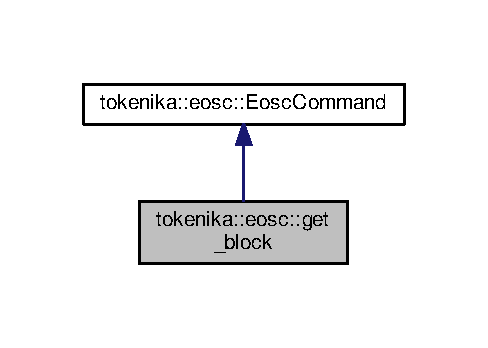
\includegraphics[width=187pt]{classtokenika_1_1eosc_1_1get__block__inherit__graph}
\end{center}
\end{figure}


Collaboration diagram for tokenika\+:\+:eosc\+:\+:get\+\_\+block\+:\nopagebreak
\begin{figure}[H]
\begin{center}
\leavevmode
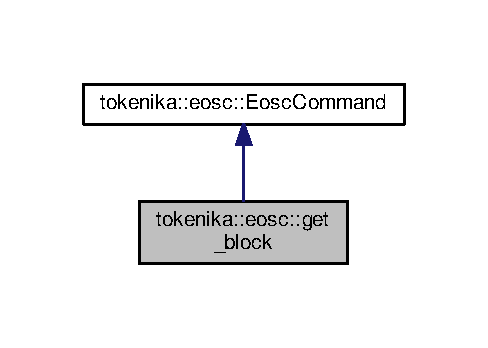
\includegraphics[width=187pt]{classtokenika_1_1eosc_1_1get__block__coll__graph}
\end{center}
\end{figure}
\subsection*{Public Member Functions}
\begin{DoxyCompactItemize}
\item 
\mbox{\Hypertarget{classtokenika_1_1eosc_1_1get__block_a8d6bd95d65d6bd8265dc3fb23e5e0350}\label{classtokenika_1_1eosc_1_1get__block_a8d6bd95d65d6bd8265dc3fb23e5e0350}} 
{\bfseries get\+\_\+block} (boost\+::property\+\_\+tree\+::ptree post\+\_\+json, bool raw=false)
\end{DoxyCompactItemize}
\subsection*{Additional Inherited Members}


\subsection{Detailed Description}
Retrieve a full block from a blockchain. 

Given a {\ttfamily boost\+::property\+\_\+tree\+::ptree json}, like (\href{#https://github.com/EOSIO/eosjs-json/blob/master/api/v1/chain.json}{\tt after eosjs-\/json}) \begin{DoxyVerb}* {"block_num_or_id":"uint32 | string"}.
* \end{DoxyVerb}


the constructor posts it to an E\+OS block socket, specified in the {\ttfamily eosc\+\_\+config.\+json} file. The responce of the blockchain is, again, a {\ttfamily boost\+::property\+\_\+tree\+::ptree json}. On error, the reaponce json is \textquotesingle{}\{\char`\"{}error\char`\"{}\+:\char`\"{}error message\char`\"{}\}, otherwise it is like (\href{#https://github.com/EOSIO/eosjs-json/blob/master/api/v1/chain.json}{\tt after eosjs-\/json}) \begin{DoxyVerb}* {
* "previous":"uint32",
* "timestamp":"2017-07-18T20:16:36",
* "transaction_merkle_root":"uint32",
* "producer":"uint16",
* "producer_changes":"map<account_name, account_name>[]",
* "producer_signature":"signature",
* "cycles":"thread[]",
* "id":"fixed_bytes33",
* "block_num":"uint32",
* "refBlockPrefix":"uint32"
* }
* \end{DoxyVerb}


It is available with the tokenika\+::eosc\+::eosc\+\_\+command\+::get\+\_\+resp\+\_\+json() method.

Note that time is a string. For processing, it has to be expressed as a structure and afterwords back to a string. Helper functions, namely tokenika\+::eosc\+::strToTime(const std\+::string).

Example\+:

\begin{DoxyVerb}* #include <stdio.h>
* #include <stdlib.h>
* #include <iostream>
* #include <string>
* #include <boost/property_tree/ptree.hpp>
* #include "EoscCommands/eosc_get_commands.hpp"  
* 
* int main(int argc, char *argv[])
* {
* boost::property_tree::ptree postJson;
* postJson.put("block_num_or_id", 25);
* tokenika::eosc::GetBlock GetBlock(GetInfo_post_json);
* std::cout << GetBlock.get<int>("last_irreversible_block_num")) << std::endl;
* boost::property_tree::ptree rcv_json = GetBlock.getRcvJson();
* std::cout << GetBlock.toStringRcv() << std::endl; // Print the response json.
* 
* return 0;
* }
* \end{DoxyVerb}
 

The documentation for this class was generated from the following file\+:\begin{DoxyCompactItemize}
\item 
eosc\+\_\+commands/eosc\+\_\+get\+\_\+commands.\+hpp\end{DoxyCompactItemize}

\hypertarget{classtokenika_1_1eosc_1_1get__block__options}{}\section{tokenika\+:\+:eosc\+:\+:get\+\_\+block\+\_\+options Class Reference}
\label{classtokenika_1_1eosc_1_1get__block__options}\index{tokenika\+::eosc\+::get\+\_\+block\+\_\+options@{tokenika\+::eosc\+::get\+\_\+block\+\_\+options}}


Inheritance diagram for tokenika\+:\+:eosc\+:\+:get\+\_\+block\+\_\+options\+:
% FIG 0


Collaboration diagram for tokenika\+:\+:eosc\+:\+:get\+\_\+block\+\_\+options\+:
% FIG 1
\subsection*{Public Member Functions}
\begin{DoxyCompactItemize}
\item 
\mbox{\Hypertarget{classtokenika_1_1eosc_1_1get__block__options_a9e525acf9a7ebe91ce8d27edfdd88a88}\label{classtokenika_1_1eosc_1_1get__block__options_a9e525acf9a7ebe91ce8d27edfdd88a88}} 
{\bfseries get\+\_\+block\+\_\+options} (int argc, const char $\ast$$\ast$argv)
\end{DoxyCompactItemize}
\subsection*{Protected Member Functions}
\begin{DoxyCompactItemize}
\item 
\mbox{\Hypertarget{classtokenika_1_1eosc_1_1get__block__options_a4bbbc3a59f550c1b82abe56be743d922}\label{classtokenika_1_1eosc_1_1get__block__options_a4bbbc3a59f550c1b82abe56be743d922}} 
const char $\ast$ {\bfseries get\+\_\+usage} ()
\item 
\mbox{\Hypertarget{classtokenika_1_1eosc_1_1get__block__options_ad0734aa9d509a4b3465b6bc4e3bbbf69}\label{classtokenika_1_1eosc_1_1get__block__options_ad0734aa9d509a4b3465b6bc4e3bbbf69}} 
virtual boost\+::program\+\_\+options\+::options\+\_\+description {\bfseries options} ()
\item 
\mbox{\Hypertarget{classtokenika_1_1eosc_1_1get__block__options_ac1d672107af6d977f72b3a8c24792859}\label{classtokenika_1_1eosc_1_1get__block__options_ac1d672107af6d977f72b3a8c24792859}} 
virtual void {\bfseries set\+\_\+pos\+\_\+desc} (boost\+::program\+\_\+options\+::positional\+\_\+options\+\_\+description \&pos\+\_\+desc)
\item 
\mbox{\Hypertarget{classtokenika_1_1eosc_1_1get__block__options_a220d34ce4b86ec412d1ac1543cbd1417}\label{classtokenika_1_1eosc_1_1get__block__options_a220d34ce4b86ec412d1ac1543cbd1417}} 
virtual bool {\bfseries set\+\_\+json} (boost\+::program\+\_\+options\+::variables\+\_\+map \&vm)
\item 
\mbox{\Hypertarget{classtokenika_1_1eosc_1_1get__block__options_a1ffc7685f937a5798197d3a22d5e6378}\label{classtokenika_1_1eosc_1_1get__block__options_a1ffc7685f937a5798197d3a22d5e6378}} 
virtual \hyperlink{classtokenika_1_1eosc_1_1eosc__command}{eosc\+\_\+command} {\bfseries get\+\_\+command} (bool is\+\_\+raw)
\item 
\mbox{\Hypertarget{classtokenika_1_1eosc_1_1get__block__options_a273ea349b38fea0dd35da0c5d774f718}\label{classtokenika_1_1eosc_1_1get__block__options_a273ea349b38fea0dd35da0c5d774f718}} 
virtual void {\bfseries get\+\_\+output} (\hyperlink{classtokenika_1_1eosc_1_1eosc__command}{eosc\+\_\+command} command)
\item 
\mbox{\Hypertarget{classtokenika_1_1eosc_1_1get__block__options_a8dcb19e3758d22b7a574617caf5afc82}\label{classtokenika_1_1eosc_1_1get__block__options_a8dcb19e3758d22b7a574617caf5afc82}} 
virtual void {\bfseries get\+\_\+example} ()
\end{DoxyCompactItemize}
\subsection*{Protected Attributes}
\begin{DoxyCompactItemize}
\item 
\mbox{\Hypertarget{classtokenika_1_1eosc_1_1get__block__options_aa0c185f1cca1b55170b63064649e9984}\label{classtokenika_1_1eosc_1_1get__block__options_aa0c185f1cca1b55170b63064649e9984}} 
int {\bfseries n}
\item 
\mbox{\Hypertarget{classtokenika_1_1eosc_1_1get__block__options_aefad040bfca5dbb07d27383fa0e0ee1f}\label{classtokenika_1_1eosc_1_1get__block__options_aefad040bfca5dbb07d27383fa0e0ee1f}} 
std\+::string {\bfseries id}
\end{DoxyCompactItemize}


The documentation for this class was generated from the following file\+:\begin{DoxyCompactItemize}
\item 
eosc\+\_\+commands/eosc\+\_\+get\+\_\+commands.\+hpp\end{DoxyCompactItemize}

\hypertarget{classtokenika_1_1eosc_1_1get__info}{}\section{tokenika\+:\+:eosc\+:\+:get\+\_\+info Class Reference}
\label{classtokenika_1_1eosc_1_1get__info}\index{tokenika\+::eosc\+::get\+\_\+info@{tokenika\+::eosc\+::get\+\_\+info}}


Get current blockchain information.  




{\ttfamily \#include $<$eosc\+\_\+get\+\_\+commands.\+hpp$>$}



Inheritance diagram for tokenika\+:\+:eosc\+:\+:get\+\_\+info\+:
% FIG 0


Collaboration diagram for tokenika\+:\+:eosc\+:\+:get\+\_\+info\+:
% FIG 1
\subsection*{Public Member Functions}
\begin{DoxyCompactItemize}
\item 
\mbox{\Hypertarget{classtokenika_1_1eosc_1_1get__info_a599f4636f791bdba2a6a34ead1b33823}\label{classtokenika_1_1eosc_1_1get__info_a599f4636f791bdba2a6a34ead1b33823}} 
{\bfseries get\+\_\+info} (const char $\ast$post\+\_\+json, bool raw=false)
\item 
\mbox{\Hypertarget{classtokenika_1_1eosc_1_1get__info_a914fda993ac1eb04e30bddac398d9253}\label{classtokenika_1_1eosc_1_1get__info_a914fda993ac1eb04e30bddac398d9253}} 
{\bfseries get\+\_\+info} (boost\+::property\+\_\+tree\+::ptree post\+\_\+json, bool raw=false)
\end{DoxyCompactItemize}
\subsection*{Additional Inherited Members}


\subsection{Detailed Description}
Get current blockchain information. 

\#include $<$stdio.\+h$>$ \#include $<$stdlib.\+h$>$ \#include $<$iostream$>$ \#include $<$string$>$ \#include \char`\"{}eosc\+\_\+commands/eosc\+\_\+get\+\_\+commands.\+hpp\char`\"{}

int main(int argc, char $\ast$argv\mbox{[}$\,$\mbox{]}) \{ \hyperlink{classtokenika_1_1eosc_1_1get__info}{tokenika\+::eosc\+::get\+\_\+info} \hyperlink{classtokenika_1_1eosc_1_1get__info}{get\+\_\+info}; // Call \textquotesingle{}eosd\textquotesingle{} for \textquotesingle{}get info\textquotesingle{}. std\+::cout $<$$<$ get\+\_\+info.\+to\+\_\+string\+\_\+rcv() $<$$<$ std\+::endl; // Print the response. return 0; \} 

The documentation for this class was generated from the following file\+:\begin{DoxyCompactItemize}
\item 
eosc\+\_\+commands/eosc\+\_\+get\+\_\+commands.\+hpp\end{DoxyCompactItemize}

\hypertarget{classtokenika_1_1eosc_1_1get__info__options}{}\section{tokenika\+:\+:eosc\+:\+:get\+\_\+info\+\_\+options Class Reference}
\label{classtokenika_1_1eosc_1_1get__info__options}\index{tokenika\+::eosc\+::get\+\_\+info\+\_\+options@{tokenika\+::eosc\+::get\+\_\+info\+\_\+options}}


Inheritance diagram for tokenika\+:\+:eosc\+:\+:get\+\_\+info\+\_\+options\+:
% FIG 0


Collaboration diagram for tokenika\+:\+:eosc\+:\+:get\+\_\+info\+\_\+options\+:
% FIG 1
\subsection*{Public Member Functions}
\begin{DoxyCompactItemize}
\item 
\mbox{\Hypertarget{classtokenika_1_1eosc_1_1get__info__options_ae17ddadfaae5f911806245ee343a7fe8}\label{classtokenika_1_1eosc_1_1get__info__options_ae17ddadfaae5f911806245ee343a7fe8}} 
{\bfseries get\+\_\+info\+\_\+options} (int argc, const char $\ast$$\ast$argv)
\end{DoxyCompactItemize}
\subsection*{Protected Member Functions}
\begin{DoxyCompactItemize}
\item 
\mbox{\Hypertarget{classtokenika_1_1eosc_1_1get__info__options_a45505a16a760f2a46a4abca28e8c3f36}\label{classtokenika_1_1eosc_1_1get__info__options_a45505a16a760f2a46a4abca28e8c3f36}} 
const char $\ast$ {\bfseries get\+\_\+usage} ()
\item 
\mbox{\Hypertarget{classtokenika_1_1eosc_1_1get__info__options_a53a235123f4c3e44714dfc9a73408b68}\label{classtokenika_1_1eosc_1_1get__info__options_a53a235123f4c3e44714dfc9a73408b68}} 
virtual bool {\bfseries set\+\_\+json} (boost\+::program\+\_\+options\+::variables\+\_\+map \&vm)
\item 
\mbox{\Hypertarget{classtokenika_1_1eosc_1_1get__info__options_a26d7097258a69f23293d23421fab84b0}\label{classtokenika_1_1eosc_1_1get__info__options_a26d7097258a69f23293d23421fab84b0}} 
virtual \hyperlink{classtokenika_1_1eosc_1_1eosc__command}{eosc\+\_\+command} {\bfseries get\+\_\+command} (bool is\+\_\+raw)
\item 
\mbox{\Hypertarget{classtokenika_1_1eosc_1_1get__info__options_aaae5074a608521882b86b8271f2296b9}\label{classtokenika_1_1eosc_1_1get__info__options_aaae5074a608521882b86b8271f2296b9}} 
virtual void {\bfseries get\+\_\+output} (\hyperlink{classtokenika_1_1eosc_1_1eosc__command}{tokenika\+::eosc\+::eosc\+\_\+command} command)
\item 
\mbox{\Hypertarget{classtokenika_1_1eosc_1_1get__info__options_a9410f7f01675b4333fed426a01f84163}\label{classtokenika_1_1eosc_1_1get__info__options_a9410f7f01675b4333fed426a01f84163}} 
virtual void {\bfseries get\+\_\+example} ()
\end{DoxyCompactItemize}
\subsection*{Additional Inherited Members}


The documentation for this class was generated from the following file\+:\begin{DoxyCompactItemize}
\item 
eosc\+\_\+commands/eosc\+\_\+get\+\_\+commands.\+hpp\end{DoxyCompactItemize}

\hypertarget{structtokenika_1_1eosc_1_1init__get1}{}\section{tokenika\+:\+:eosc\+:\+:init\+\_\+get1 Struct Reference}
\label{structtokenika_1_1eosc_1_1init__get1}\index{tokenika\+::eosc\+::init\+\_\+get1@{tokenika\+::eosc\+::init\+\_\+get1}}
\subsection*{Data Fields}
\begin{DoxyCompactItemize}
\item 
\mbox{\Hypertarget{structtokenika_1_1eosc_1_1init__get1_a16f6c66fce8c542e8523b10148ddc835}\label{structtokenika_1_1eosc_1_1init__get1_a16f6c66fce8c542e8523b10148ddc835}} 
std\+::string {\bfseries str\+Val}
\item 
\mbox{\Hypertarget{structtokenika_1_1eosc_1_1init__get1_a3bbaa7577047893fea408af7bc26d3a6}\label{structtokenika_1_1eosc_1_1init__get1_a3bbaa7577047893fea408af7bc26d3a6}} 
int {\bfseries int\+Val}
\item 
\mbox{\Hypertarget{structtokenika_1_1eosc_1_1init__get1_a51a3770c50aebba378d7068951ecfe62}\label{structtokenika_1_1eosc_1_1init__get1_a51a3770c50aebba378d7068951ecfe62}} 
float {\bfseries float\+Val}
\item 
\mbox{\Hypertarget{structtokenika_1_1eosc_1_1init__get1_a0f3e1707874a60d3b60bfc8809d5fe6f}\label{structtokenika_1_1eosc_1_1init__get1_a0f3e1707874a60d3b60bfc8809d5fe6f}} 
boost\+::posix\+\_\+time\+::ptime {\bfseries ptime}
\end{DoxyCompactItemize}


The documentation for this struct was generated from the following file\+:\begin{DoxyCompactItemize}
\item 
eosc\+\_\+command.\+cpp\end{DoxyCompactItemize}

%--- End generated contents ---

% Index
\backmatter
\newpage
\phantomsection
\clearemptydoublepage
\addcontentsline{toc}{chapter}{Index}
\printindex

\end{document}
